% !TeX root = er.tex

\chapter{Mapping}\label{ch.mapping}
\index{mapping}

\abstract*{A robot uses a map to localize its position. Maps can be loaded into the robot, but often the robot must create a map by itself. Maps are represented using either a grid showing which cells are occupied and which are free or a continuous map containing the coordinates of the obstacles. For a grid map the frontier algorithm enables the robot to explore its environment in order to determine the probability that each cell is occupied or free. A robot can use knowledge of its environment, for example, that it is in a building with rectangular rooms, to facilitate building a map. Algorithms for simultaneous localization and mapping enable a robot to perform these two tasks together, using data from localization and its sensor to extend the map and data from the map to achieve accurate localization.}

We have seen that a robot can use its capability to detect obstacles to localize itself, based on information about the position of the obstacles or other information on the environment. This information is normally provided by a map. It is relatively easy to construct a map of industrial environments such as factories, since the machines are anchored in fixed locations. Maps are less relevant for a robotic vacuum cleaner, because the manufacturer cannot prepare maps of the apartments of every customer. Furthermore, the robots would be too difficult to use if customers had to construct maps of their apartments and change them whenever a piece of furniture is moved. It goes without saying that it is impossible to construct in advance maps of inaccessible locations like the ocean floor.

The solution is to have the robot build its own map of the environment. To build a map requires localization so that the robot knows where it is, but localization needs a map, which needs \ldots. To overcome this chicken-and-egg problem, robots use \emph{simultaneous localization and mapping (SLAM)}\index{simultaneous localization and mapping (SLAM)} algorithms. To perform SLAM robots use information known to be valid even in unexplored parts of the environment, refining the information during the exploration.

This is what humans did to create geographic maps. Observations of the sun and stars were used for localization and maps were created as exploration proceeded. Initially, tools for localization were poor: it is relatively easy to measure latitude using a sextant to observe the height of the sun at noon, but accurate measurements of longitude were impossible until accurate clocks called chronometers were developed in the late eighteenth century. As localization improved so did maps, including not only land and seacoasts, but also terrain features like lakes, forests and mountains, as well as artificial structures like buildings and roads.

Sections~\ref{s.maps}--\ref{s.grids} introduce methods of representing maps in a computer. Section~\ref{s.map-create} describes how a robot can create a map using the frontier algorithm. Section~\ref{s.map-update} explains how partial knowledge of the environment helps in constructing a map. A SLAM algorithm is the subject of the final three sections.  The algorithm is first presented in Sect.~\ref{s.slam-numerical} using a relatively simple example. Activities for SLAM are collected in Sect.~\ref{s.slam-activities} and Sect.~\ref{s.slam-formal} explains the formal algorithm.

\section{Discrete and continuous maps}\label{s.maps}

We are used to graphical maps that are printed on paper, or, more commonly these days, displayed on computers and smartphones. A robot, however, needs a non-visual representation of a map that it can store in its memory. There are two techniques for storing maps: discrete maps (also called \emph{grid maps}\index{map!grid}) and continuous maps.

Figure~\ref{fig.disc} shows an $8\times 8$ grid map with a triangular object. The location of the object is stored as a list of the coordinates of each grid cell covered by the object. The object in the figure consists of the cells at:
\[
(5,3),\, (5,4),\, (5,5)\,, (4,5)\,, (5,6),\, (4,6),\, (3,6)\,.
\]

\begin{figure}
\subfigures
\begin{minipage}{\textwidth}
\leftfigure[c]{
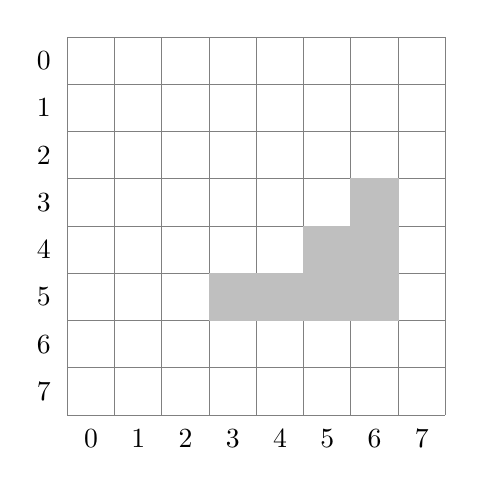
\begin{tikzpicture}[scale=1.2]
\draw[step=5mm,gray] (0,0) grid (4,4);
\foreach \r in {0,1,2,3,4,5,6,7}
  \node at (-.25,3.75-\r*.5) {$\r$};
\foreach \c in {0,1,2,3,4,5,6,7}
  \node at (.25+\c*.5,-.25) {$\c$};
\foreach \x/\y in {3/2, 4/2, 5/2, 6/2, 5/3, 6/3, 6/4}
   \draw[fill,gray!50] (\x/2,\y/2) rectangle +(5mm,5mm);
\path (4.1,0) -- (4.1,4.1); % Avoid truncation
\end{tikzpicture}
}
\hspace{\fill}
\rightfigure[c]{
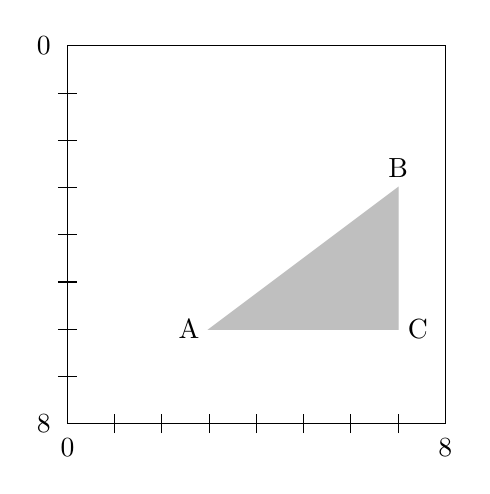
\begin{tikzpicture}[scale=1.2]
\draw (0,0) rectangle +(4,4);
\node at (-.25,0) {$8$};
\node at (-.25,4) {$0$};
\node at (0,-.25) {$0$};
\node at (4,-.25) {$8$};
\foreach \x in {1,2,3,4,5,6,7}
  \draw (\x*.5,-.1) -- (\x*.5,.1);
\foreach \y in {1,2,3,4,5,6,7}
  \draw (-.1,\y*.5) -- (.1,\y*.5);
\draw[fill,gray!50] (3/2,2/2) node[black,left] {\p{A}} -- (7/2,2/2) node[black,right] {\p{C}} -- (7/2,5/2) node[black,above] {\p{B}} -- cycle;
\path (4.1,0) -- (4.1,4.1); % Avoid truncation
\end{tikzpicture}
}
\leftcaption{A discrete map of the occupied cells of an object}\label{fig.disc}
\rightcaption{A continuous map of the same object\label{fig.cont}}
\end{minipage}
\end{figure}

Figure~\ref{fig.cont} shows a \emph{continuous map}\label{map!continuous} of the same object. Instead of storing the positions of the object, the coordinates of boundary positions are stored:
\[A = (6,3),\, B = (3,7),\, C = (6,7)\,.
\]

Discrete maps are not very accurate: it is hard to recognize the object in Fig.~\ref{fig.disc} as a triangle. To improve accuracy, a finer grid must be used: $16\times 16$ or even $256\times 256$. Of course, as the number of grid points increases, so must the size of the memory in the robot. In addition, a more powerful computer must be used to process the grid cells. Mobile robots have constraints on weight, cost, battery capacity, and so on, so very fine grids may not be practical. 

If the objects in the environment are few and have a simple shape, a continuous map is more efficient, in addition to being more accurate. In Fig.~\ref{fig.cont}, three pairs of numbers represent the triangle with far greater accuracy than the seven pairs of the discrete map. Furthermore, it is easy to compute if a point is in the object or not using analytic geometry. However, if there are many objects or if they have very complex shapes, continuous maps are no longer efficient either in memory or in the amount of computation needed. The object in Fig.~\ref{fig.cont} is bounded by straight lines, but if the boundary were described by high-order curves, the computation would become difficult. Consider a map with $32$ objects of size one, none of which touch each other. The discrete map would have $32$ coordinates, while the continue map would need to store the coordinates of the four corners of each object.

In mobile robotics, discrete maps are commonly used to represent maps of environments, as we did in Chap.~\ref{ch.local}.

\section{The content of the cells of a grid map}\label{s.grids}
\index{map!encoding}

A geographic map uses conventional notations to describe the environment. Colors are used: green for forests, blue for lakes, red for highways. Symbols are used: dots of various sizes to denote villages and towns, and lines for roads, where the thickness and color of a line is used to indicate the quality of the road. Robots use grid maps where each cell stores a number and we need to decide what a number encodes.

The simplest encoding is to allocate one bit to each cell. A value of $1$ indicates that an object exists in that cell and a value of $0$ indicates that the cell is empty. In Fig.~\ref{fig.disc}, gray represents the value $1$ and white represents the value $0$.

However, sensors are not accurate and it may be difficult to be certain if a cell is occupied by an object or not. Therefore, it makes sense to assign a probability to each cell indicating how certain we are that the object is in that cell. Figure~\ref{fig.prob-grid} is a copy of Fig.~\ref{fig.disc} with the probabilities listed for each cell. Cells without a number are assumed to have a probability of $0$.

\begin{figure}
\begin{center}
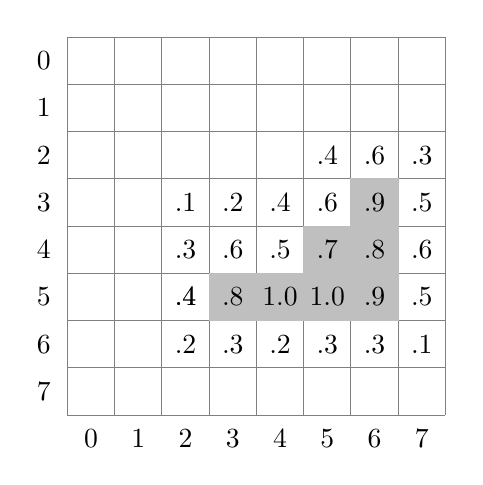
\begin{tikzpicture}[scale=1.2]
\draw[step=5mm,gray] (0,0) grid (4,4);
\foreach \r in {0,1,2,3,4,5,6,7}
  \node at (-.25,3.75-\r*.5) {$\r$};
\foreach \c in {0,1,2,3,4,5,6,7}
  \node at (.25+\c*.5,-.25) {$\c$};
\foreach \x/\y in {3/2, 4/2, 5/2, 6/2, 5/3, 6/3, 6/4}
   \draw[fill,gray!50] (\x/2,\y/2) rectangle +(5mm,5mm);
\foreach \x/\y/\p in {3/2/$.8$, 4/2/$1.0$, 5/2/$1.0$, 6/2/$.9$, 5/3/$.7$, 6/3/$.8$, 6/4/$.9$, 2/2/$.4$, 2/2/$.4$, 2/3/$.3$, 3/3/$.6$, 4/3/$.5$, 5/4/$.6$, 3/4/$.2$, 4/4/$.4$, 2/4/$.1$, 5/5/$.4$, 6/5/$.6$, 7/5/$.3$, 7/4/$.5$, 7/3/$.6$, 7/2/$.5$, 7/1/$.1$, 6/1/$.3$, 5/1/$.3$, 4/1/$.2$, 3/1/$.3$, 2/1/$.2$ }
   \node at (\x/2+.25,\y/2+.25) {\p};
\path (4.1,0) -- (4.1,4.1); % Avoid truncation
\end{tikzpicture}
\caption{A probabilistic grid map}\label{fig.prob-grid}
\end{center}
\end{figure}

It can be seen that cells with a probability of at least $.7$ are the ones considered in Fig.~\ref{fig.disc} to be cells occupied by the object. Of course, we are free to choose some other threshold, for example $.5$, in which case more cells are considered to be occupied. In this example, we know that the object is triangular, so we can see that a threshold of $.5$ makes the object bigger than it actually is, while the higher threshold $.7$ gives a better approximation.

\begin{framed}
\act{Probabilistic map of obstacles}{obstacle-map}
\begin{itemize}
\item Place your robot on a line in front of a set of obstacles that the robot can detect with a lateral sensor (Fig.~\ref{fig.mapping-activity}). If you implemented localization as described in Activity~\ref{act.local-uncertain}, you can use this information to establish where the robot is. Otherwise, draw regular lines on the ground that can be read by the robot for localization. Build a probabilistic map of the obstacles.
\item How do the probabilities change when obstacles are added or removed?
\end{itemize}
\end{framed}

\begin{figure}
\begin{center}
\begin{tikzpicture}
\draw[fill,lightgray] (-1,-2.5mm) rectangle +(8,5mm);
\pic[scale=1.2] at (0,-5mm) { robot2 };
\foreach \x in {-10mm, 5mm, 20mm, 35mm, 50mm, 65mm}
  \draw[fill,lightgray] (\x,-12mm) rectangle +(3mm,6mm);
\draw[fill] (5,1) rectangle +(12mm,5mm);
\draw[fill] (2,1) rectangle +(12mm,5mm);
\draw[dashed,thick] (15mm,4mm) -- +(20:10mm);
\draw[dashed,thick] (12mm,5mm) -- +(100:10mm);
\end{tikzpicture}
\end{center}
\caption{The black rectangles are the obstacles to be measured. The gray line guides the robot and the gray marks are used for localization}\label{fig.mapping-activity}
\end{figure}

\section{Creating a map by exploration: The frontier algorithm}\label{s.map-create}
\index{mapping!exploring the environment}

Consider a robotic vacuum cleaner newly let loose in your apartment. Obviously, it does not come pre-programmed with a map of your apartment. Instead, it must explore the environment to gather information that will be used to construct its own map. There are several ways of exploring the environment, the simplest of which is random exploration. The exploration will be much more efficient if the robot has a partial map that it can use to guide its exploration.

\subsection{Grid maps with occupancy probabilities}

The map in Fig.~\ref{fig.map-explore} is a grid map where each cell is labeled with its \emph{obstacle probability}\index{mapping!occupancy probability}, which is the probability that there is an obstacle in the cell. The obstacle can be a wall, a table or anything that does not allow the robot to pass through this cell. The question marks represent cells that have not yet been explored. In the absence of any knowledge about the contents of a cell, we can assume that the probability that there is an obstacle there is $0.5$, since it could just as easily be occupied or not. A question mark is used instead of the value $0.5$ to clarify the unexplored status of the cells.

\begin{figure}
\begin{center}
\includegraphics[width=\textwidth]{grid-mapping1.pdf}
\end{center}
\caption{Grid map of an environment with occupancy probabilities}\label{fig.map-explore}
\end{figure}

The center of the map is free from obstacles and the occupancy probabilities of these cells, called \emph{open cells}, are low ($0.1$ or $0.2$). There are three known obstacles, at the top right, the top left and the bottom center. The obstacles are characterized by high occupancy probabilities ($0.9$ or $1.0$) and are denoted by gray cells. A \emph{frontier cell} is an open cell that is adjacent (left, right, up, down) to one or more unknown cells. The set of frontier cells is called the \emph{frontier}. The red lines of small squares in Fig.~\ref{fig.map-explore} represent the boundary between the frontier and the unknown cells in the environment. The unknown cells adjacent to the frontier are the interesting ones that should be explored in order to expand the current map.

\subsection{The frontier algorithm}

The \emph{frontier algorithm}\index{mapping!frontier algorithm} is used to expand the map by exploring the frontier. The robot moves to the closest frontier cell, senses if there are obstacles in unknown adjacent cells and updates the map accordingly. 

The grid map in Fig.~\ref{fig.map-explore1} is the same as the map in Fig.~\ref{fig.map-explore} with the addition of the robot which occupies a cell colored blue. The frontier cell closest to the robot is the cell two steps above its initial location. The arrow shows that the robot has moved to that cell. The robot uses its local sensors to determine if there are obstacles in adjacent unknown cells. (The sensors can detect obstacles in all eight adjacent cells, including the ones on the diagonal.) Suppose that the cell to its upper left certainly contains an obstacle (probability $1.0$), while the cells directly above and to the right almost certainly do not contain an obstacle (probability $0.1$). Figure~\ref{fig.map-explore2} shows the map updated with this new information and the new position of the frontier.


\begin{figure}
\begin{center}
\includegraphics[width=\textwidth]{grid-mapping1b.pdf}
\end{center}
\caption{The robot moves to the frontier}\label{fig.map-explore1}
\end{figure}

\begin{figure}
\begin{center}
\includegraphics[width=\textwidth]{grid-mapping1c.pdf}
\end{center}
\caption{The robot updates unknown cells adjacent to the frontier}\label{fig.map-explore2}
\end{figure}

Figure~\ref{fig.map-explore3} shows the result of the next iteration of the algorithm. The robot has moved up one cell to the closest frontier cell, detected obstacles in the two adjacent unknown cells and updated the map. The upper right obstacle is completely known and there is no frontier cell in the vicinity of the current position of the robot.

\begin{figure}
\begin{center}
\includegraphics[width=\textwidth]{grid-mapping1d.pdf}
\end{center}
\caption{Second iteration of the frontier algorithm}\label{fig.map-explore3}
\end{figure}

Figure~\ref{fig.map-explore4} shows the next iteration of the algorithm. The robot is blocked by the upper right obstacle and has to avoid it as it moves to the nearest frontier cell.

Figure~\ref{fig.map-explore5} shows the completed map constructed by the robot after it has explored the entire frontier as shown by the path with the blue arrows. 

Algorithm~\ref{alg.frontier} formalizes the frontier algorithm. For simplicity, the algorithm recomputes the frontier at each step. A more sophisticated algorithm would examine the cells in a neighborhood of the robot's position and add or remove the cells whose status as frontier cells has changed.

The example to which we applied the frontier algorithm is a relatively simple environment consisting of two rooms connected by a door (at the sixth column from the left in Fig.~\ref{fig.map-explore5}), but otherwise closed to the outside environment. However, the frontier algorithm works in more complex environments. 

\begin{figure}
\begin{center}
\includegraphics[width=\textwidth]{grid-mapping1e.pdf}
\end{center}
\caption{The robot avoids an obstacle while moving to the next frontier}\label{fig.map-explore4}
\end{figure}

\begin{figure}
\begin{center}
\includegraphics[width=\textwidth]{grid-mapping1f.pdf}
\end{center}
\caption{The map constructed by the frontier algorithm and the path explored by the robot}\label{fig.map-explore5}
\end{figure}

\begin{figure}
\begin{alg}{Frontier algorithm}{frontier}
\hline
&\idv{}float array grid&// Grid map\\
&\idv{}cell list frontier&// List of frontier cells\\
&\idv{}cell robot& // Cell with robot\\
&\idv{}cell closest&// Closest cell to robot\\
&\idv{}cell c&// Index over cells\\
&\idv{}float low&// Low occupancy probability\\
\hline
\stl{}&loop&\\
\stl{}&\idc{}frontier \ass{} empty&\\
\stl{}&\idc{}for all known cells c  in the grid&\\
\stl{}&\idc{}\idc{}if grid(c) $<$ low and&\\
\stl{}&\idc{}\idc{}\idc{}exists unknown neighbor of c&\\
\stl{}&\idc{}\idc{}\idc{}\idc{}append c to frontier&\\
\stl{}&\idc{}exit if frontier empty&\\
&&\\
\stl{}&\idc{}closest \ass{} cell in frontier nearest robot&\\
\stl{}&\idc{}robot \ass{} closest&\\
\stl{}&\idc{}for all unknown neighbors c of closest&\\
\stl{}&\idc{}\idc{}\idc{}sense if c is occupied&\\
\stl{}&\idc{}\idc{}\idc{}mark grid(c) with occupancy probability&\\
\end{alg}
\end{figure}

The frontier algorithm can be run in parallel by multiple robots. Each robot will explore that portion of the frontier that is closest to its position. The robots share their partial maps so that consistency of the maps is maintained. Since each robot explores a different area of the environment, the construction of the map will be much more efficient.

\subsection{Priority in the frontier algorithm}\label{s.priority}

The frontier algorithm can use criteria other than distance to choose which frontier to explore. Consider the exploration of the grid map shown in Fig.~\ref{fig.map-seven}. The robot is at cell $(3,3)$ marked with the blue circle. There are six known obstacle cells and five known open cells, of which the three cells $(1,3), (2,2), (3,2)$, marked with red squares, are the frontier cells. (Here the diagonal neighbors are not considered as adjacent.)

\begin{figure}
\begin{center}
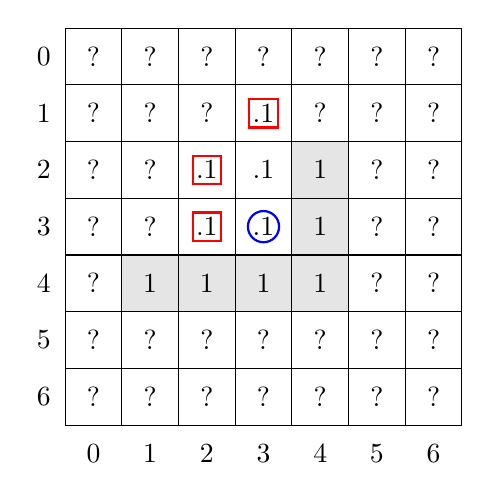
\begin{tikzpicture}[scale=.9]
% Obstacles
\foreach \r/\c in {32/32, 32/24, 32/16, 8/16, 16/16, 24/16}
  \fill[gray!20] (\r mm,\c mm) rectangle +(8mm,8mm);
% Robot
%\fill[gray!50] (24mm,24mm) rectangle +(8mm,8mm);
\draw[blue,thick] (28mm,28mm) circle [radius=2.2mm];
% Frontier
\foreach \r/\c in {18/26, 18/34, 26/42}
  \draw[red,thick] (\r mm,\c mm) rectangle +(4mm,4mm);
% Grid
\draw[step=8mm] (0,0) grid (56mm,56mm);
\foreach \r in {0,1,2,3,4,5,6} {
  \node at (\r*8mm+4mm,-4mm) {\p{\r}};
}
\foreach \r in {0,1,2,3,4,5,6} {
  \node at (-3mm,52mm-\r*8mm) {\p{\r}};
}
% Cells
\foreach \r in {0,1,2,3,4,5,6} {
  \node at (\r*8mm+4mm,52mm) {\p{?}};
}
\foreach \r/\a in {0/?,1/?,2/?,3/.1,4/?,5/?,6/?} {
  \node at (\r*8mm+4mm,44mm) {\p{\a}};
}
\foreach \r/\a in {0/?,1/?,2/.1,3/.1,4/1,5/?,6/?} {
  \node at (\r*8mm+4mm,36mm) {\p{\a}};
}
\foreach \r/\a in {0/?,1/?,2/.1,3/.1,4/1,5/?,6/?} {
  \node at (\r*8mm+4mm,28mm) {\p{\a}};
}
\foreach \r/\a in {0/?,1/1,2/1,3/1,4/1,5/?,6/?} {
  \node at (\r*8mm+4mm,20mm) {\p{\a}};
}
\foreach \r in {0,1,2,3,4,5,6} {
  \node at (\r*8mm+4mm,12mm) {\p{?}};
}
\foreach \r in {0,1,2,3,4,5,6} {
  \node at (\r*8mm+4mm,4mm) {\p{?}};
}
\end{tikzpicture}
\caption{Exploration of a labyrinth}\label{fig.map-seven}
\end{center}
\end{figure}

In Algorithm~\ref{alg.frontier}, the robot uses distance to a frontier cell as the criterion for deciding where to move. In Fig.~\ref{fig.map-seven} the cell to the robot's left at $(3,2)$ is the closest cell since it is only one step away, while the other two frontier cells are two steps away. We can consider a different criterion by taking into account the number of unknown cells adjacent to a frontier cell. Starting with a frontier cell with more unknown cells might make the algorithm more efficient. We define the priority of a frontier cell as:
\[
p_\sub{cell} = \frac{a_\sub{cell}}{d_\sub{cell}}\,,
\]
where $a_\sub{cell}$ is the number of adjacent unknown cells and $d_\sub{cell}$ is the distance from the robot. The priorities of the three frontier cells are:
\[
p_{(3,2)} = 1/1 = 1,\;\;p_{(2,2)} = 2/2 = 1,\;\;p_{(1,3)} = 3/2 = 1.5\,.
\]
The priority of cell $(1,3)$ is the highest and the exploration starts there.

\begin{framed}
\act{Frontier algorithm}{frontier}
\begin{itemize}
\item Implement the frontier algorithm. You will need to include an algorithm to move accurately from one cell to another and an algorithm to move around obstacles.
\item Run the program on the grid map in Fig.~\ref{fig.map-explore5}. Do you get the same path? If not, why not?
\item Run the program on the grid map in Fig.~\ref{fig.map-seven}.
\item Modify Algorithm~\ref{alg.frontier} to use the priority described in Sect.~\ref{s.priority}. Is the path different from the one generated by the original program?
\item Try to implement the frontier algorithm on your robot. What is the most difficult aspect of the implementation?
\end{itemize}
\end{framed}

\section{Mapping using knowledge of the environment}\label{s.map-update}
\index{mapping!knowledge of the environment@{with knowledge of the environment}}

Now that we know how to explore an environment, let us consider how to build a map during the exploration. In Chap.~\ref{ch.local} we saw that a robot can localize itself with the help of external landmarks and their representation in a map. Without such external landmarks, the robot can only rely on odometry or inertial measurement, which are subject to errors that increase with time (Fig.~\ref{fig.odo-errors}). How is it possible to make a map when localization is subject to large errors?

Even with bad odometry, the robot can construct a better map if it has some information on the structure of the environment. Suppose that the robot tries to construct the plan of a room by following its walls. Differences in the real speeds of the left and right wheels will lead the robot to conclude that the walls are not straight (Fig.~\ref{fig.map-room1}), but if the robot knows \emph{in advance} that the walls are straight and perpendicular to each other, the robot can construct the map shown in Fig.~\ref{fig.map-room2}. When it encounters a sharp turn, it understands that the turn is a $90^\circ$ corner where two walls meet, so its mapping of the angles will be correct. There will also be an error when measuring the lengths of the walls and this can lead to the gap shown in the figure between the first and last walls. The figure shows a small gap which would not be important, but if the robot is mapping a large area, the problem of \emph{closing a loop}\index{simultaneous localization and mapping (SLAM)!closing the loop} in a map is hard to solve because the robot has only a local view of the environment.


\begin{figure}
\subfigures
\begin{minipage}{\textwidth}
\leftfigure{
\begin{tikzpicture}[scale=1.2]
\pic[rotate=90,scale=.5] at (0,0) { robot };
\draw[bend right=10] (-6mm,0mm) to (-10mm,25mm);
\draw[bend right=10] (-10mm,25mm) to (10mm,35mm);
\draw[bend right=10] (10mm,35mm) to (25mm,20mm);
\draw[bend right=10] (25mm,20mm) to (20mm,5mm);
\end{tikzpicture}
}
\hspace{\fill}
\rightfigure{
\begin{tikzpicture}[scale=1.2]
\pic[rotate=90,scale=.5] at (0,0) { robot };
\draw (-6mm,2mm)  to (-6mm,25mm);
\node at (-8mm,0mm) {\p{gap}};
\draw (-6mm,25mm) to (20mm,25mm);
\draw (20mm,25mm) to (20mm,-4mm);
\draw (20mm,-4mm) to (-6mm,-4mm);
\draw (-6mm,-4mm) to (-6mm,-2mm);
\end{tikzpicture}
}
\leftcaption{Perceived motion of a robot based on odometry }\label{fig.map-room1}
\rightcaption{Odometry together with knowledge of the geometry of the walls}\label{fig.map-room2}
\end{minipage}
\end{figure}

Consider a robotic lawnmower given the task of mowing a lawn by moving back and forth; it has to close the loop by returning to its charging station (Fig.~\ref{fig.lawn}). It is not possible to implement this behavior using odometry alone, since small errors in velocity and heading lead to large errors in the position of the robot. It is highly unlikely that through odometry alone the robot will mow the entire surface of the lawn and return to its charging station. Landmarks such as signaling cables in the ground need to be used to close the loop.

\begin{figure}
\begin{center}
% Robotic lawnmower
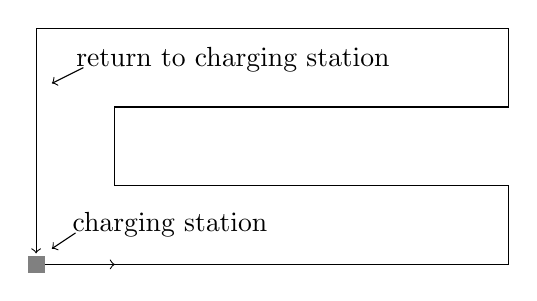
\begin{tikzpicture}[align=left]
\node at (2.5,2.6) {\p{return to charging station}};
\draw[->] (.6,2.5) -- +(-4mm,-2mm);
\draw (0,0) -- (6,0) -- (6,1) -- (1,1) -- (1,2) -- (6,2) -- (6,3) -- (0,3);
\draw[->] (0,0) -- (1,0);
\draw[->] (0,3) -- (0,4pt);
\draw[fill,gray] (-1mm,-1mm) rectangle +(2mm,2mm);
\node at (1.7,.5) {\p{charging station}};
\draw[->] (.5,.4) -- +(-3mm,-2mm);
\end{tikzpicture}
\end{center}
\caption{A robotic lawnmower mowing an area and returning to its charging station}\label{fig.lawn}
\end{figure}

Map construction can be significantly improved by using sensor data that can give information on regular features in the environment, in particular, at a long range. The regular features can be lines on the ground, a global orientation, or the detection of features that \emph{overlap}\index{simultaneous localization and mapping (SLAM)!overlap} with other measurements. Suppose that we have a distance sensor that can measure distances over a large area (Fig.~\ref{fig.map_overlap}). The measurement over a large area enables the robot to identify features such as walls and corners from a measurement taken at a single location. Large area measurements facilitate identifying overlaps between the local maps that are constructed at each location as the robot moves through the environment. By comparing local maps, the localization can be corrected and map accurately updated. This is the topic of the SLAM algorithm described in the next section.

\begin{figure}
\begin{center}
\begin{tikzpicture}[scale=1.2]
\pic[rotate=90,scale=.5] at (0,0) { robot };
\pic[rotate=90,scale=.5] at (0,19mm) { robot };
\pic[scale=.5] at (10mm,28mm) { robot };
\draw[thick,dashed,color=red] (0,2mm) circle[radius=14mm];
\draw[thick,dashed,color=blue] (0,21mm) circle[radius=14mm];
\draw[thick,dashed,color=green!70!black] (12mm,28mm) circle[radius=14mm];
\draw[thick,color=red,yshift=-2pt] (-6mm,-10mm) -- (-6mm,15mm);
\draw[thick,color=blue] (-7mm,9mm) -- (-7mm,33mm) -- (8mm,33mm);
\draw[thick,color=green!70!black] (-1mm,34mm) -- (25mm,34mm);
\end{tikzpicture}
\end{center}
\caption{Long range sensor measurements can detect overlap}\label{fig.map_overlap}
\end{figure}

\begin{framed}
\act{Robotic lawnmower}{lawnmower}
\begin{itemize}
\item Write a program that causes a robotic lawnmower to move along a path using odometry alone (Fig.~\ref{fig.lawn}). Run the program several times. Does the robot return to the charging station? If not, how large are the errors? Are the errors consistent or do they change from one run to the next?
\item Place landmarks of black tape around the lawn (Fig.~\ref{fig.lawn-landmarks}). Program your robot to recognize the landmarks and correct its localization. How large do the landmarks have to be so that the robot detects them reliably?
\end{itemize}
\end{framed}

\begin{figure}
\begin{center}
% Robotic lawnmower with landmarks
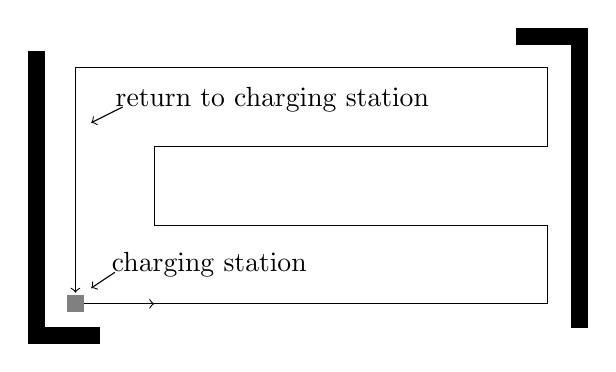
\begin{tikzpicture}[align=left]
\node at (2.5,2.6) {\p{return to charging station}};
\draw[->] (.6,2.5) -- +(-4mm,-2mm);
\draw (0,0) -- (6,0) -- (6,1) -- (1,1) -- (1,2) -- (6,2) -- (6,3) -- (0,3);
\draw[->] (0,0) -- (1,0);
\draw[->] (0,3) -- (0,4pt);
\draw[fill,gray] (-1mm,-1mm) rectangle +(2mm,2mm);
\node at (1.7,.5) {\p{charging station}};
\draw[->] (.5,.4) -- +(-3mm,-2mm);
\draw[fill,black] (-.6,-.4) rectangle +(2mm,3.6);
\draw[fill,black] (-.6,-.5) rectangle +(9mm,2mm);
\draw[fill,black] (6.3,-.3) rectangle +(2mm,3.6);
\draw[fill,black] (6.5,3.3) rectangle +(-9mm,2mm);
\end{tikzpicture}
\end{center}
\caption{A robotic lawnmower with landmarks}\label{fig.lawn-landmarks}
\end{figure}

\section{A numerical example for a SLAM algorithm}\label{s.slam-numerical}
\index{simultaneous localization and mapping (SLAM)!numerical example}

The SLAM algorithm is quite complicated so we first compute a numerical example and later give the formal presentation.

Figure~\ref{fig.mapping1a} shows a robot in a room heading towards the top of the diagram. The robot is near a corner of the room and there is a projection from the wall to the robot's left, perhaps a supporting pillar of the building. Fig.~\ref{fig.mapping1b} is the corresponding map. The large dot shows the position of the robot and the associated arrow shows its heading. The thick dotted line represents the real wall. The white cells represent locations that are known to be free, the gray cells represent obstacles, and the cells with question marks are still unexplored. A cell is considered to be part of the obstacle if a majority of the area of the cell is behind the wall. For example, the two horizontal segments of the projection from the wall are near the boundary of the cells they pass through, but these cells are considered part of the obstacle because almost all their area is behind the wall.

\begin{figure}
\subfigures
\begin{minipage}{\textwidth}
\leftfigure{
\includegraphics[width=.4\textwidth]{mappingA.pdf}
}
\hspace{\fill}
\rightfigure{
\includegraphics[width=.4\textwidth]{mappingB.pdf}
}
\leftcaption{A robot near the wall of a room}\label{fig.mapping1a}
\rightcaption{The corresponding map}\label{fig.mapping1b}
\end{minipage}
\end{figure}

For the purpose of presenting the details of the SLAM algorithm, the map is highly simplified. First, the cells are much too large, roughly the same size as the robot itself. In practice, the cells would be much smaller than the robot. Second, we specify that each (explored) cell is either free (white) or it contains an obstacle (gray); real SLAM algorithms use a probabilistic representation (Sect.~\ref{s.grids}).

Suppose that the robot in Fig.~\ref{fig.mapping1a} intends to move forwards to the new position shown in Fig.~\ref{fig.mapping2a}. Figure~\ref{fig.mapping2b} shows the map corresponding to the position after the intended move, where the robot has moved the height of one cell up from its initial position. Unfortunately, the right wheel moves over an area of low friction and although the robot ends up in the correct position, its heading is too far to the right. The actual position of the robot is shown in  Fig.~\ref{fig.mapping2c} and Fig.~\ref{fig.mapping2d} is the corresponding map.

\begin{figure}
\subfigures
\begin{minipage}{\textwidth}
\leftfigure{
\includegraphics[width=.43\textwidth]{mapping2A.pdf}
}
\hspace{\fill}
\rightfigure{
\includegraphics[width=.43\textwidth]{mapping2B.pdf}
}
\leftcaption{The intended motion of the robot}\label{fig.mapping2a}
\rightcaption{The map for the intended motion}\label{fig.mapping2b}
\end{minipage}
\end{figure}

\begin{figure}
\subfigures
\begin{minipage}{\textwidth}
\leftfigure{
\includegraphics[width=.43\textwidth]{mapping2C.pdf}
}
\hspace{\fill}
\rightfigure{
\includegraphics[width=.43\textwidth]{mapping2D.pdf}
}
\leftcaption{The actual motion of the robot}\label{fig.mapping2c}
\rightcaption{The map for the actual motion}\label{fig.mapping2d}
\end{minipage}
\end{figure}

Figure~\ref{fig.mapping3a} (which is the same as Fig.~\ref{fig.mapping2b}) shows the \emph{intended} perception of the robot because the robot has moved one cell upwards relative to the map in Fig.~\ref{fig.mapping1b}. From this position it can detect the obstacle to its left and investigate the unknown cells in front of it.

However, because of the error in odometry, the \emph{actual} perception of the robot is different. Figure~\ref{fig.mapping3b} shows the actual position of the wall as seen by the robot overlaid on top of the cells, where cells are colored gray if the majority of their area is known to be behind the wall. (Examine several cells to verify that this is true.) We assume that the robot can sense walls at a distance of up to five times the size of a cell as shown by the dashed circle and we also assume that the robot knows that any wall is one cell thick.

\begin{figure}
\subfigures
\begin{minipage}{\textwidth}
\leftfigure{
\includegraphics[width=.43\textwidth]{mapping3A.pdf}
}
\hspace{\fill}
\rightfigure{
\includegraphics[width=.43\textwidth]{mapping3B.pdf}
}
\leftcaption{The intended perception of the robot}\label{fig.mapping3a}
\rightcaption{The actual perception of the robot}\label{fig.mapping3b}
\end{minipage}
\end{figure}

There is a clear mismatch between the current map and the sensor data which should correspond to the known part of the map. Obviously, the robot is not where it is expected to be based on odometry. How can this mismatch be corrected? We assume that odometry does give a reasonable estimation of the pose (position and heading) of the robot. For each relatively small possible error in the pose, we compute what the perception of the current map would be and compare it with the actual perception computed from the sensor data. The pose that gives the best match is chosen as the actual pose of the robot and the current map updated accordingly.

In the example, assume that the robot is either in the expected cell or in one of its four neighbors (left, right, up, down) and that the heading of the robot is either correct or turned slightly to the right ($15^\circ$ clockwise (CW)) or slightly to the left ($15^\circ$  counterclockwise (CCW)). The $5\times 3=15$ possible poses are shown in Fig.~\ref{fig.pos-explore} and Fig.~\ref{fig.mapping4} shows the perception of the map computed from the current map for each pose. (To save space, only a $8\times 5$ fragment of the $12\times 8$ map is displayed.)

\begin{figure}
\begin{center}
\includegraphics[width=0.5\textwidth]{pos-explore.pdf}
\end{center}
\caption{Possible poses of the robot}\label{fig.pos-explore}
\end{figure}

\begin{figure}
\begin{center}
\includegraphics[width=0.9\textwidth]{mapping4b.pdf}
\end{center}
\caption{Estimations of perception of the robot for different poses}\label{fig.mapping4}
\end{figure}

The next step is to choose the map that gives the best fit with the sensor measurements. First transform the $8\times 5$ maps into $8\times 5$ matrices, assigning $-1$ to empty cells, $+1$ to obstacle cells and $0$ to other cells. The left matrix in Fig.~\ref{fig.mapping5} is associated with the current map and the center matrix in the figure is associated with the perception map corresponding to the pose where the robot is in the correct cell but the heading is $15^\circ$ CW (the middle element of the top row of Fig.~\ref{fig.mapping4}).

To compare the maps, multiply elements of corresponding cells. Let $m(i,j)$ be the $(i,j)$'th cell of the current map and $p(i,j)$ be the $(i,j)$'th cell of the perception map obtained from sensor values. $S(i,j)$, the \emph{similarity} of $(i,j)$'th cell, is:
\[
S(i,j) = m(i,j)\, p(i,j)\,,
\]
which can also be expressed as:
\[
\begin{array}{l@{\hspace{2em}}l}
S(i,j) = 1 & \textrm{if}\;\;m(i,j) \neq 0,\, p(i,j) \neq 0,\, m(i,j) = p(i,j)\\
S(i,j) = -1 & \textrm{if}\;\;m(i,j) \neq 0,\, p(i,j) \neq 0,\,  m(i,j) \neq p(i,j)\\
S(i,j) = 0 & \textrm{if }m(i,j) = 0\, \textrm{or}\; p(i,j) = 0\,.
\end{array}
\]
The right matrix in Fig.~\ref{fig.mapping5} shows the result of this computation for the two matrices to its left. There are a lot of $1$'s meaning that the matrices are similar and thus we can conclude that the perception maps are similar. For a quantitative result, compute the sum of the similarities to obtain a single value for any pair $m,p$:
\[
\mathcal{S} = \sum_{i=1}^8 \sum_{j=1}^5 S(i,j)\,.
\]

\begin{figure}
\begin{center}
\includegraphics[width=\textwidth]{mapping5.pdf}
\end{center}
\caption{Computation of the matching between two maps}\label{fig.mapping5}
\end{figure}

Table~\ref{tab.matching} gives the values of the similarity $\mathcal{S}$ for all the perception maps in Fig.~\ref{fig.mapping4} compared with the current map. As expected, the highest similarity is obtained for the map corresponding to the pose with the correct position and with the heading rotated by $15^\circ$ CW.

\begin{table}
\caption{Similarity $\mathcal{S}$ of the sensor-based map with the current map}
\label{tab.matching}
\renewcommand{\arraystretch}{1.2}
\setlength{\tabcolsep}{8pt}
\begin{tabular}{p{22mm}ccc}
\svhline\noalign{\smallskip}
&Intended orientation&$15^{\circ}$ CW&$15^{\circ}$ CCW\\
Intended position & $22$ & \boldmath $32$ & $20$\\
Up one cell       & $23$ & $25$ & $16$\\
Down one cell     & $19$ & $28$ & $21$\\
Left one cell     & $6$  & $7$  & $18$\\
Right one cell    & $22$ & $18$ & $18$\\
\noalign{\smallskip}\svhline\noalign{\smallskip}
\end{tabular}
\end{table}

Once we have this result, we correct the pose of the robot and use data from the perception map to update the current map stored in the robot's memory (Fig.~\ref{fig.final-map}).

\begin{figure}
\begin{center}
\includegraphics[width=\textwidth]{final-map.pdf}
\end{center}
\caption{Map before and after the update using data from the perception map}\label{fig.final-map}
\end{figure}
\medskip

\section{Activities for demonstrating the SLAM algorithm}\label{s.slam-activities}

The following two activities demonstrate aspects of the SLAM algorithm. Activity~\ref{act.computed-perceptions} follows the algorithm and is intended for implementation in software. Activity~\ref{act.measured-perceptions} demonstrates a key element of the algorithm that can be implemented on an educational robot.

The activities are based on the configuration shown in Fig.~\ref{fig.slam-config}. The robot is located at the origin of the coordinate system with pose $((x,y),\theta)=((0,0),0^\circ)$.\footnote{It is convenient to take the heading of the robot as $0^\circ$.} Given the uncertainty of the odometry, the robot might actually be located at any of the coordinates $(-1,0), (1,0), (0,-1), (0,1)$ and its orientation might be any of $-15^\circ, 0, -15^\circ$ (as shown by the dashed arrows), giving $15$ possible poses. The three gray dots at coordinates $(2,2), (2,0), (2,-2)$ represent known obstacles on the current map. (To save space the dots are displayed at coordinates $(2,1), (2,0), (2,-1)$.) The obstacles can be sensed by multiple horizontal proximity sensors, but for the purposes of the activities we specify that there are three sensors.

\begin{figure}
\begin{center}
% SLAM algorithm
\begin{tikzpicture}
\draw[step=3cm,very thin,gray] (-3.01,-3.01) grid (6,3);
% The obstacles
\fill[gray!80!black] (6,0) circle[radius=6pt];
\fill[gray!80!black] (6,3) circle[radius=6pt];
\fill[gray!80!black] (6,-3) circle[radius=6pt];
% The robots
\pic at (0,0) { robot };
\pic at (3,0) { robot };
\pic at (-3,0) { robot };
\pic at (0,3) { robot };
\pic at (0,-3) { robot };
% The three arrows on each robot
\foreach \x/\y in {0/0, 3/0, -3/0, 0/3, 0/-3} {
  \draw[dashed,->,thick] (\x,\y) -- +( 20:15mm);
  \draw[dashed,->,thick] (\x,\y) -- +(  0:15mm);
  \draw[dashed,->,thick] (\x,\y) -- +(-20:15mm);
}
\node at (-3.6,-2.9) {$(-1,-1)$};
\node at (3,3.3) {$(1,1)$};
\end{tikzpicture}
\caption{Configuration for the SLAM algorithm}\label{fig.slam-config}
\end{center}
\end{figure}

In the SLAM algorithm the \emph{perception} of an obstacle is the value returned by a distance sensor. To avoid having to define model for the sensors, the activities will define a perception as the \emph{distance} and \emph{heading} from the sensor to the obstacle.

\begin{framed}
\act{Localize the robot from the computed perceptions}{computed-perceptions}
\begin{itemize}
\item For each of the $15$ poses compute the set of perceptions of each obstacle. For example, if the robot is at the pose $((0.0,1.0),-15.0^\circ)$, the set of perceptions of the three obstacles is:
\[
[( 2.2,  41.6^\circ),\,  ( 2.2, -11.6^\circ),\,  ( 3.6, -41.3^\circ)]\,.
\]
\item Given a set of measured perceptions, compute their similarities to the perceptions of the $15$ poses of the robot. Choose the pose with the best similarity as the actual pose of the robot. For example, for the set of measured perceptions:
\[
[( 2.0,  32.0^\circ),\,  ( 2.6, -20.0^\circ),\,  ( 3.0, -30.0^\circ)]\,,
\]
and the similarity computed as the sum of the absolute differences of the elements of the perceptions, the pose with the best similarity is $((0.0, 1.0),-15.0^\circ)$.
\item Experiment with different similarity functions.
\item We have computed that the robot's pose is approximately $((0.0, 1.0),-15.0^\circ)$. Suppose that a new obstacle is placed at coordinate $(3,0)$. Compute the perception $(d,\theta)$ of the object from this pose and then compute the coordinate $(x,y)$ of the new obstacle. The new obstacle can be added to the map with this coordinate.
\item Is the computed coordinate significantly different from the coordinate $(3,0)$ that would be obtained if the robot were at its intended pose $((0,0),0^\circ)$?
\end{itemize}
\end{framed}

\begin{framed}
\act{Localize the robot from the measured perceptions}{measured-perceptions}
\begin{itemize}
\item Place three objects as shown in Fig.~\ref{fig.slam-config}.
\item Write a program that stores the set of values returned by the three horizontal proximity sensors. Place your robot successively at each of the $15$ poses and record the sets of values. You now have a database of perceptions: a set of three sensor readings for each pose.
\item Place the robot at one of the poses and store the set of values returned by the sensors. Compute the  similarity of this set to each of the sets in the database. Display the pose associated with the best similarity.
\item Experiment with placing the robot at various poses and several times at each pose. How precise is the determination of the pose?
\item Experiment with different similarity functions.
\end{itemize}
\end{framed}

\section{The formalization of the SLAM algorithm}\label{s.slam-formal}
\index{simultaneous localization and mapping (SLAM)!algorithm}

Algorithm~\ref{alg.slam} is a SLAM algorithm that finds the position whose perception map is closest to the perception map obtained from the sensor data. The robot is localized to this position and the map updated to what is perceived at this position.

\begin{figure}
\begin{alg}{SLAM}{slam}
\hline
&\idv{}matrix $\vec{m}$ \ass partial map&// Current map\\
&\idv{}matrix $\vec{p}$&// Perception map\\
&\idv{}matrix $\vec{e}$&// Expected map\\
&\idv{}coordinate $\vec{c}$ \ass initial position&// Current position\\
&\idv{}coordinate $\vec{n}$&// New position\\
&\idv{}coordinate array $\vec{T}$&// Set of test positions\\
&\idv{}coordinate $\vec{t}$&// Test position\\
&\idv{}coordinate $\vec{b}$ \ass none&// Best position\\
\hline
\stl{}&loop&\\
\stl{}&\idc{}move a short distance&\\
\stl{}&\idc{}$\vec{n}$ \ass odometry($\vec{c}$)&// New position based on odometry\\
\stl{}&\idc{}$\vec{p}$ \ass analyze sensor data&\\
&&\\
\stl{}&\idc{}for every $\vec{t}$ in $\vec{T}$&// T is the positions around n\\
\stl{}&\idc{}\idc{}$\vec{e}$ \ass expected($\vec{m}$, $\vec{t}$)&// Expected map at test position\\
\stl{}&\idc{}\idc{}if compare($\vec{t}$,$\vec{e}$) better than $\vec{b}$&\\
\stl{}&\idc{}\idc{}\idc{}$\vec{b}$ \ass $\vec{t}$&// Best test position so far\\
&&\\
\stl{}&\idc{}$\vec{n}$ \ass $\vec{b}$&// Replace new position by best position\\
\stl{}&\idc{}$\vec{m}$ \ass update($\vec{m}$,$\vec{p}$,$\vec{n})$&// Update map based on new position\\
\stl{}&\idc{}$\vec{c}$ \ass $\vec{n}$&// Current position is new position\\
\end{alg}
\end{figure}

The algorithm is divided into three phases. In the first phase (lines~2--4), the robot moves a short distance and its new position is computed by odometry. The perception map at this location is obtained by analyzing the sensor data.

Assuming that the odometry error is relatively small, we can define a set of test positions where the robot might be. In the second phase (lines~5--8), the expected map at each of these positions is computed and compared with the current map. The best match is saved.

In the third phase (lines~9--11), the position with the best match becomes the new position and the current map is updated accordingly.

In practice, the algorithm is somewhat more complicated because it has to take into account that the perception map obtained from the sensors is limited by the range of the sensors. The overlap will be partial both because the sensor range does not cover the entire current map and because the sensors can detect obstacles and free areas outside the current map. Therefore, the size of the perceived map $\vec{p}$ will be much smaller than the expected map $\vec{e}$ and the function \p{compare(}$\vec{p}$\p{,}$\vec{e}$\p{)} will only compare the areas that overlap. Furthermore, when updating the current map, areas not previously in the map will be added. In Fig.~\ref{fig.final-map} there are cells in the current map that are outside the five-cell radius of the sensor and will not be updated. The light red cells were unknown in the current map as indicated by the question marks, but in the perception map they are now known to be part of the obstacle. This information is used to update the current map to obtain a new current map.

\section{Summary}

Accurate robotic motion in an uncertain environment requires that the robot have a map of the environment. The map must be maintained in the robot's computer; it can be either a grid map of cells or a graph representation of a continuous map. In an uncertain environment, a map will typically not be available to the robot before it begins its tasks. The frontier algorithm is used by a robot to construct a map as it explores its surroundings. More accurate maps can be constructed if the robot has some knowledge of its environment, for example, that the environment is the inside of a building consisting of rectangular rooms and corridors. Simultaneous localization and mapping (SLAM) algorithms use an iterative process to construct a map while also correcting for errors in localization.

\section{Further reading}

Two textbooks on path and motion planning are \cite{latombe,lavalle}. See also \cite[Chapter 6]{siegwart}.

The frontier algorithm was proposed by Yamauchi \cite{yamauchi} who showed that a robot could use the algorithm to successfully explore an office with obstacles.

Algorithms for SLAM use probability, in particular Bayes rule. Probabilistic methods in robotics are the subject of the textbook \cite{thrun}.

A two-part tutorial on SLAM by Durrant-Whyte and Bailey can be found in \cite{slam-tutorial1,slam-tutorial2}. A tutorial on graph-based SLAM is \cite{slam-graph}.

Sebastian Thrun's online course \emph{Artificial Intelligence for Robotics} is helpful:\par\url{https://classroom.udacity.com/courses/cs373}.

\bibliographystyle{spmpsci}
\bibliography{er}
